\documentclass{warpdoc}
\newlength\lengthfigure                  % declare a figure width unit
\setlength\lengthfigure{0.158\textwidth} % make the figure width unit scale with the textwidth
\usepackage{psfrag}         % use it to substitute a string in a eps figure
\usepackage{subfigure}
\usepackage{rotating}
\usepackage{pstricks}
\usepackage[innercaption]{sidecap} % the cute space-saving side captions
\usepackage{scalefnt}
\usepackage{bm}
\usepackage{amsmath}     
\usepackage{multirow}
\usepackage{graphicx}
\usepackage{rotating}
\usepackage{bm}
\usepackage{pdfpages}
%\usepackage{caption}
\usepackage{float}
\pdfminorversion=7

%%%%%%%%%%%%%=--NEW COMMANDS BEGINS--=%%%%%%%%%%%%%%%%%%%%%%%%%%%%%%%%%%
\newcommand{\alb}{\vspace{0.2cm}\\} % array line break
\newcommand{\ordi}{{\rm d}}
%\let\vec\bf
\renewcommand{\vec}[1]{\bm{#1}}
\newcommand{\mfa}{\scriptscriptstyle}
\newcommand{\mfb}{\scriptstyle}
\newcommand{\mfc}{\textstyle}
\newcommand{\mfd}{\displaystyle}
\newcommand{\hlinex}{\vspace{-0.34cm}~~\\ \hline \vspace{-0.31cm}~~\\}
\newcommand{\hlinextop}{\vspace{-0.46cm}~~\\ \hline \hline \vspace{-0.32cm}~~\\}
\newcommand{\hlinexbot}{\vspace{-0.37cm}~~\\ \hline \hline \vspace{-0.50cm}~~\\}
\newcommand{\tablespacing}{\vspace{-0.4cm}}
\renewcommand{\fontsizetable}{\footnotesize\scalefont{0.9}}
\setcounter{tocdepth}{3}
\let\citen\cite

%%%%%%%%%%%%%=--NEW COMMANDS ENDS--=%%%%%%%%%%%%%%%%%%%%%%%%%%%%%%%%%%%%
%%%%%%%%%%%%%=--NEW COMMANDS BEGINS--=%%%%%%%%%%%%%%%%%%%%%%%%%%%%%%%%%%


\author{
 Felipe Martín Rodríguez Fuentes
}

\email{
  fmrodriguez@arizona.edu
}

\department{
  Aerospace and Mechanical Engineering
}

\institution{
  University of Arizona
}

\title{Three Species Argon Plasma Kinetics 
}

\date{
Octorber 2025
}

%\setlength\nomenclaturelabelwidth{0.13\hsize}  % optional, default is 0.03\hsize
%\setlength\nomenclaturecolumnsep{0.09\hsize}  % optional, default is 0.06\hsize

\nomenclature{

  \begin{nomenclaturelist}{Roman symbols}
   \item[$a$] speed of sound
  \end{nomenclaturelist}
}


\abstract{
abstract
}

\begin{document}
  \pagestyle{headings}
  \pagenumbering{arabic}
  \setcounter{page}{1}
%  \maketitle
  \makewarpdoctitle
%  \makeabstract
 \tableofcontents
%  \makenomenclature
 % \listoftables
 % \listoffigures
%

\section{Overview}

% $$V(t) = V_{\rm dc} + V_{\rm rf}\cos (\omega t +\phi)$$

% $$\sigma_{\mathrm{superelastic}}(E) = 
% \frac{E + \Delta E}{E} \,
% \sigma_{\mathrm{forward}}(E + \Delta E)$$

\begin{table*}[!ht]
  \center\fontsizetable
  \begin{threeparttable}
    \tablecaption{Species included in the reaction mechanism.}
    \label{tab:species}
    \fontsizetable
 
    \begin{tabular*}{0.3\textwidth}{@{}l@{\extracolsep{\fill}}l@{}}
    
    \toprule

charged${}^-$ & $\rm e^-$\\

charged${}^+$ & $\rm Ar^+$\\
      
neutral, atomic & $\rm Ar$\\
    

    \bottomrule
    \end{tabular*}
   \end{threeparttable}
\end{table*}

This is the three species version of the argon mechanism: it is obtained from the four
species mechanism by removing the metastable $\rm Ar(4s)$ and every reaction in which it
takes part, so that the only process left is the ionization of ground state argon by
electron impact. The energy lost by the electrons to the inelastic processes other than
ionization is not accounted for here; it enters through the source term of the electron
temperature transport model, in the manner of the $-n_{\rm e} N k L$ term of Boeuf and
Pitchford \cite{pr:1995:boeuf}.



% \begin{figure}[ht]
%      \centering
%      
\includegraphics[width=0.5\textwidth]{figs/cs.pdf}
%      \caption{Relevant cross sections used for the BOLSIG+ calculations.}
%      \label{fig:cs_Ar}
% \end{figure}


\section{Argon chemical reactions}

 The list of reactions is given in Table~\ref{tab:Ar_tab}. When reaction rate data is given as a function of the reduced electric field $E/N$, this is converted to reaction rates function of electron energy (or temperature) through the characteristic Ar energy curve $E/N = f(T_{\rm e})$ at 300 K. 
 
 % \cite{ijae:2011:katsonis}, \cite{jap:1993:lymberopoulos}






\begin{figure}[ht]
     \centering
     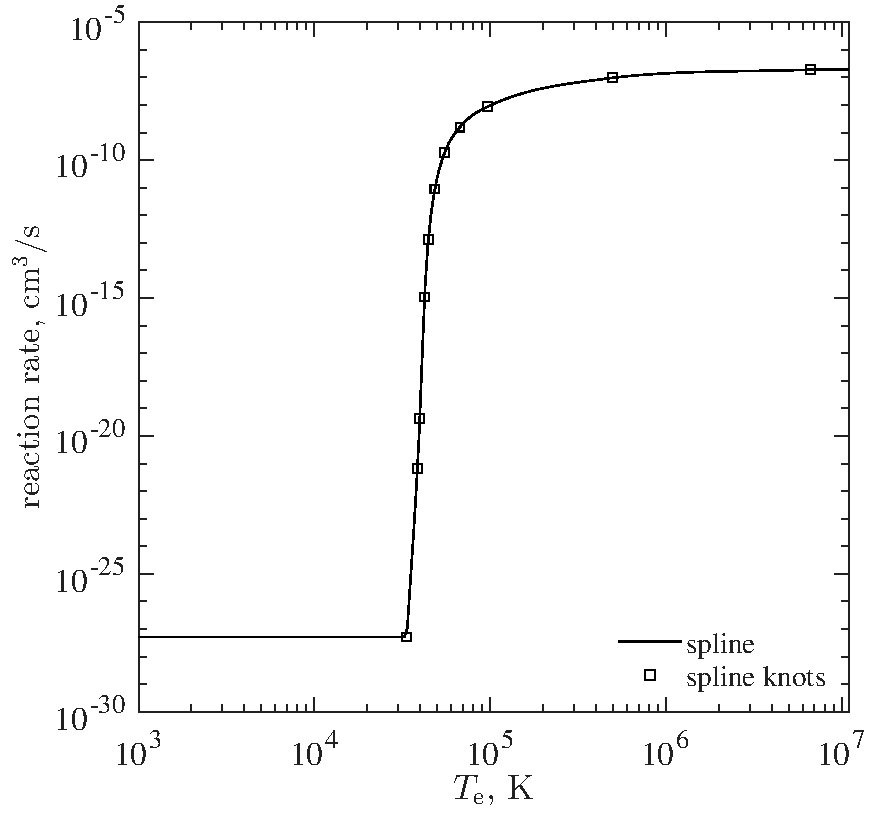
\includegraphics[width=0.5\textwidth]{figs/reaction4.pdf}
     \caption{Reaction 1: $\rm e^- + Ar \rightarrow Ar^+ + 2e^-$; comparison of ionization rate of Ar obtained with bolsigminus using cross section data from \cite{jcp:1965:rapp} at 300 K. Reference data from \cite{jap:1993:lymberopoulos}.}
     \label{fig:rate_R4}
\end{figure}






\begin{table*}[!ht]
  \center\fontsizetable
  \begin{threeparttable}
  \renewcommand{\arraystretch}{1.1}
    \tablecaption{Argon chemical kinetics\tnote{a}.}
    \label{tab:Ar_tab}
    \fontsizetable
    \begin{tabular*}{1.05\textwidth}{l@{\extracolsep{\fill}}lllccr}
    \toprule
    No.~~~~& Reaction & $T,~\textrm{K}$ & $A$  & $n$ & $E$ & Cross-section/rate ref. \\
    \midrule



  1  & $\rm e^- +Ar \rightarrow Ar^+ + e^- + e^-$
       & $T_{\rm e}$
       & \multicolumn{3}{p{6cm}}{Rate obtained with bolsigminus}       
       & \cite{jcp:1965:rapp} \\


 
    \bottomrule
    \end{tabular*}
\begin{tablenotes}
\item[{a}] The reaction rate is given by $A T^n \exp(-E/RT)$ when not presented in spline-fit form. The universal gas constant is $R = 1.987~{\rm cal~K^{-1}~mol^{-1}}.$ $N_A$ is Avogadro's number and it is approximately $6.022 \cdot 10^{23}~{\rm mol^{-1}}$. The units of $A$ are $\rm cm^3~ mol^{-1} ~s^{-1}$ for 2-body reactions and $\rm cm^6 ~mol^{-2} ~ s^{-1}$ for 3-body reactions. The units of $E$ are ${\rm cal~mol^{-1}}$.


\end{tablenotes}
   \end{threeparttable}
\end{table*}


\begin{table*}[!ht]
  \center\fontsizetable
  
  \begin{threeparttable}
    \tablecaption{Coordinates of spline control points for Argon electron impact reactions.\tnote{a}}
    \label{tab:ei_splines_Ar}
    \fontsizetable
 
    \begin{tabular*}{\textwidth}{@{}l@{\extracolsep{\fill}}lll@{}}
    
    \toprule
Process & Reaction ~ & ${\rm ln}~T_{\rm e}$ & ${\rm ln}~k$ \\
        \midrule
        

Ground ionization & ~{$\rm e^- + Ar \rightarrow Ar^+ + e^- + e^-$  } &   \begin{minipage}[t]{0.28\textwidth}\raggedright  
    10.82646
    10.96672
    10.99798
    11.06005
    11.11007
    11.19590
    11.32563
    11.52376
    11.88015
    13.52579
    16.11810
 \end{minipage}  & \begin{minipage}[t]{0.28\textwidth}\raggedright 
    -62.83592
    -48.78568
    -44.60907
    -34.45233
    -29.62413
    -25.43377
    -22.37717
    -20.26565
    -18.58446
    -16.15063
    -15.47303
\end{minipage} \\         
~\\


\alb 
    \bottomrule
    \end{tabular*}
\begin{tablenotes}
\item[{a}] The reaction rate $k$ has units of $\textrm{cm}^3\cdot \textrm{s}^{-1}$. The electron temperature $T_{\rm e}$ is in Kelvin.

\end{tablenotes}
\label{tab:reactionratessplinecontrolpoints}
   \end{threeparttable}
\end{table*}




 \clearpage
\bibliographystyle{warpdoc}
\bibliography{all}


\end{document}


